\documentclass[11pt]{article} % taille de police et type de document

\usepackage[utf8]{inputenc} % encodage des caractères
\usepackage[french]{babel} % langue du document
\usepackage[a4paper, margin=1in]{geometry} % format papier et taille de marge
\usepackage[colorlinks=true, urlcolor=blue, linkcolor=black, pdfborder={0 0 0 [0 0]}]{hyperref} % gestion des liens hypertextes (bordures invisibles)
\usepackage{color} % gestion des couleurs (\color{couleur} et \definecolor{...})
\usepackage{eurosym} % pour le symbole € (\euro)
\usepackage{graphicx} % pour inclure des images (\includegraphics[angle, scale, height, width, page]{image.png})
\usepackage{tabularx} % pour les tableaux (\begin{tabularx}{taille}{|X|X|X|})
\usepackage{listings} % pour l'inclusion de code (\lstinputlisting[language=foo]{ficher.foo})
\usepackage{wrapfig} % pour intégrer une figure dans un texte (\begin{wrapfig}{taille})
%\usepackage{showframe} % pour afficher les bordures des marges/zones de texte

\definecolor{commentcolor}{rgb}{0.50, 0.50, 0.50} % couleur grise pour les commentaires
\definecolor{forest}{rgb}{0.13, 0.55, 0.13}

\lstset{ % style des inclusions de code
	basicstyle=\footnotesize,
	frame=single,
	numbers=left,
	breaklines=true,
	showstringspaces=false,
	rulecolor=\color{black},
	commentstyle=\color{commentcolor},
	keywordstyle=\color{blue},
	stringstyle=\color{red},
	backgroundcolor=\color{white},
}

\lstset{literate=
	{á}{{\'a}}1 {é}{{\'e}}1 {í}{{\'i}}1 {ó}{{\'o}}1 {ú}{{\'u}}1
	{Á}{{\'A}}1 {É}{{\'E}}1 {Í}{{\'I}}1 {Ó}{{\'O}}1 {Ú}{{\'U}}1
	{à}{{\`a}}1 {è}{{\'e}}1 {ì}{{\`i}}1 {ò}{{\`o}}1 {ù}{{\`u}}1
	{À}{{\`A}}1 {È}{{\'E}}1 {Ì}{{\`I}}1 {Ò}{{\`O}}1 {Ù}{{\`U}}1
	{ä}{{\"a}}1 {ë}{{\"e}}1 {ï}{{\"i}}1 {ö}{{\"o}}1 {ü}{{\"u}}1
	{Ä}{{\"A}}1 {Ë}{{\"E}}1 {Ï}{{\"I}}1 {Ö}{{\"O}}1 {Ü}{{\"U}}1
	{â}{{\^a}}1 {ê}{{\^e}}1 {î}{{\^i}}1 {ô}{{\^o}}1 {û}{{\^u}}1
	{Â}{{\^A}}1 {Ê}{{\^E}}1 {Î}{{\^I}}1 {Ô}{{\^O}}1 {Û}{{\^U}}1
	{œ}{{\oe}}1 {Œ}{{\OE}}1 {æ}{{\ae}}1 {Æ}{{\AE}}1 {ß}{{\ss}}1
	{ç}{{\c c}}1 {Ç}{{\c C}}1 {ø}{{\o}}1 {å}{{\r a}}1 {Å}{{\r A}}1
	{€}{{\euro}}1 {£}{{\pounds}}1
}

\title{Projet CAD - Dossier de conception}
\author{Alexis \bsc{Lanoix} \and Jofrey \bsc{Luc} \and Quentin \bsc{Sonrel}}
\date\today

\begin{document} % début du corps du document

\maketitle

\section{Introduction}

Concernant les spécifications imposées dans le sujet, nous avons pour le moment choisi de ne pas prendre en compte la version où le joueur choisit le bateau qui effectue le tir courant.\\

Par rapport à notre conception, nous avons choisi d'utiliser un pattern MVC plutôt classique et nous utiliserons très probablement Swing pour l'interface graphique pendant la phase de développement.\\

Nous nous sommes principalement concentrés sur la partie modèle du projet et donc par conséquent la partie vue/contrôleur n'est que peu développée dans nos diagrammes mais cela nous semble normal étant donné que la décomposition des classes de ces parties n'est pas très complexe contrairement au modèle où l'interaction entre les différentes classes qui le compose est primordiale.

\newpage

\section{Diagrammes}

\begin{figure}[h!]
	\centering
	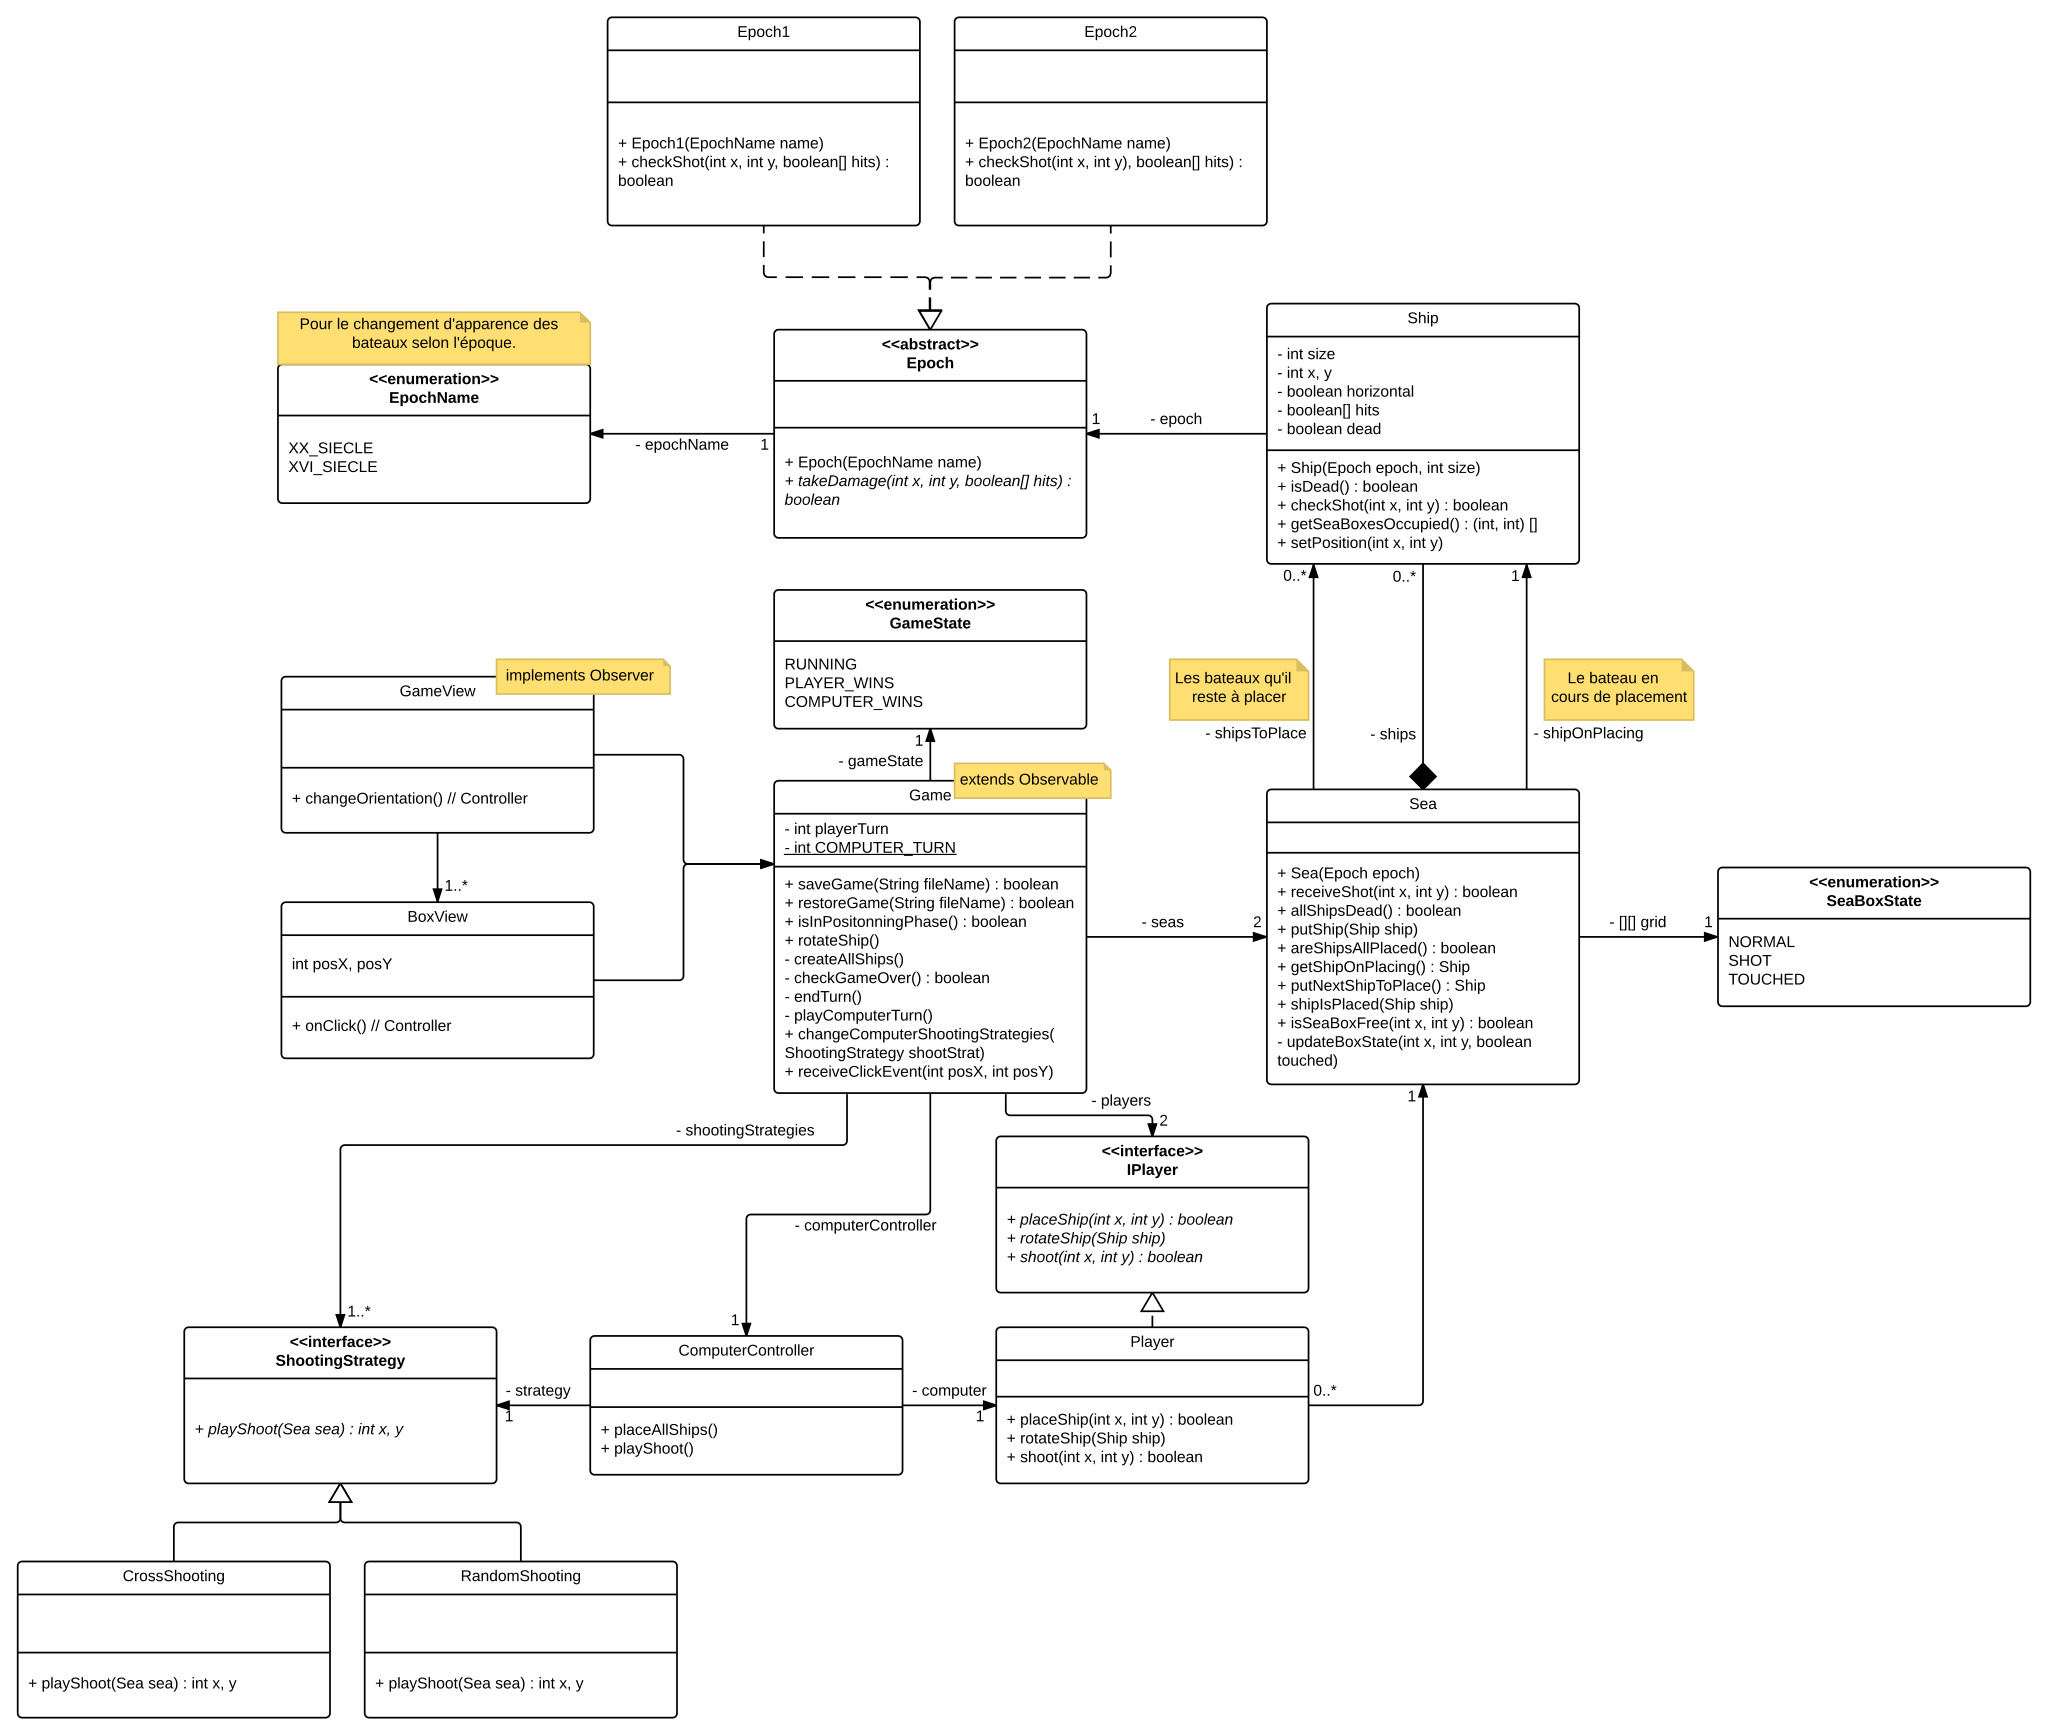
\includegraphics[angle=90, width=\textwidth]{./src/img/classes.pdf}
	\caption{Diagramme de classes}
\end{figure}

\begin{figure}[h!]
	\centering
	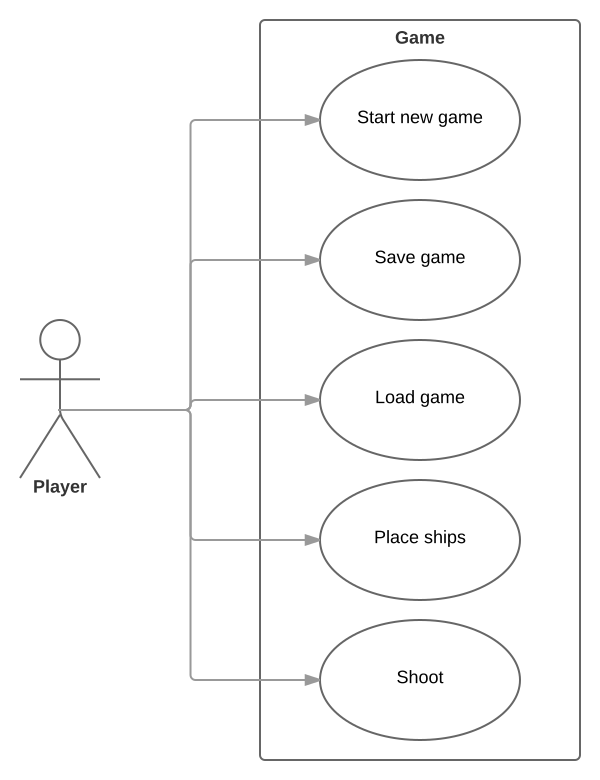
\includegraphics[width=0.7\textwidth]{./src/img/utilisation.pdf}
	\caption{Diagramme d'utilisation}
\end{figure}

\begin{figure}[h!]
	\centering
	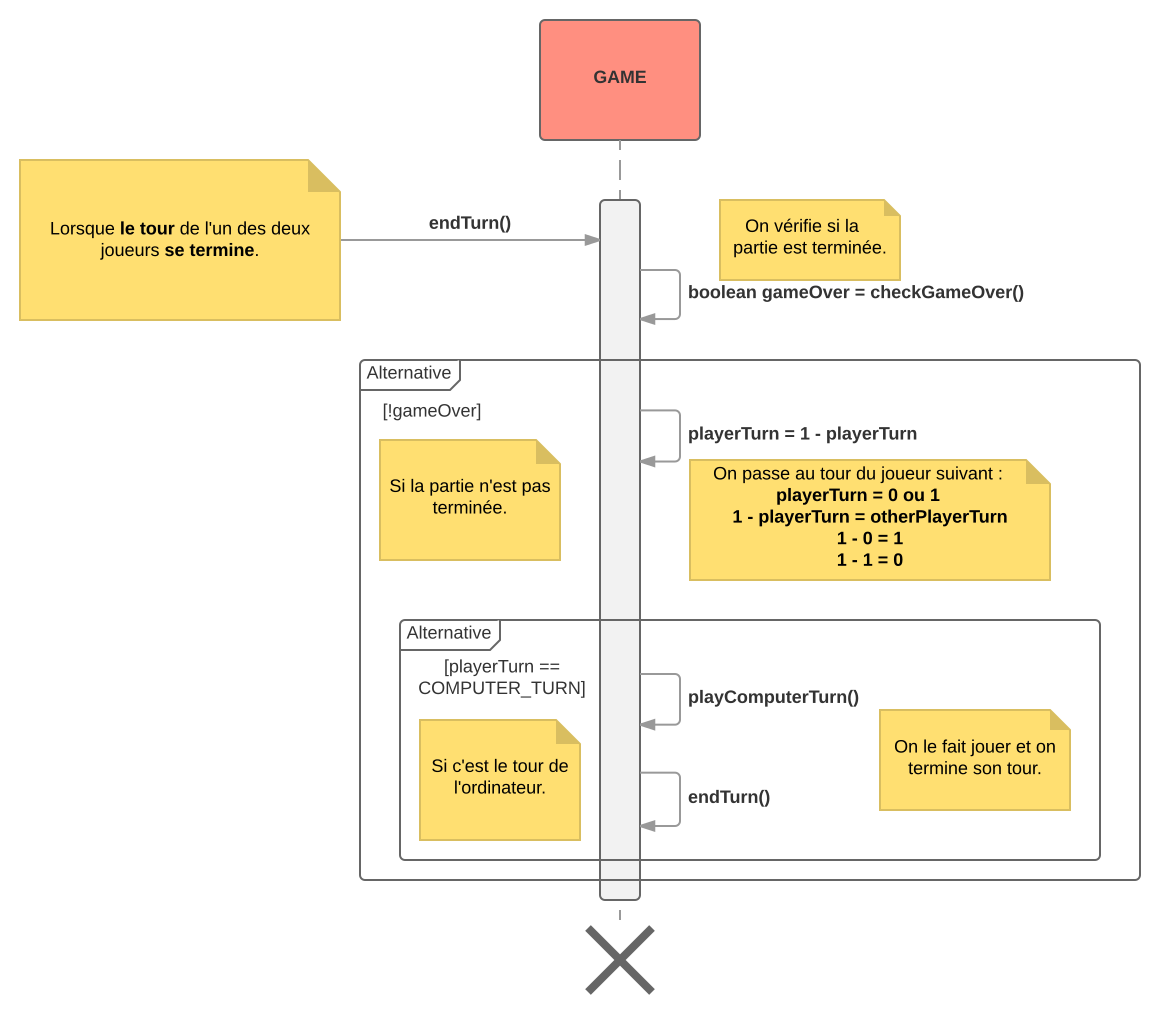
\includegraphics[angle=90, width=\textwidth]{./src/img/sequence-game-endturn.pdf}
	\caption{Diagramme de séquence - game.endTurn()}
\end{figure}

\begin{figure}[h!]
	\centering
	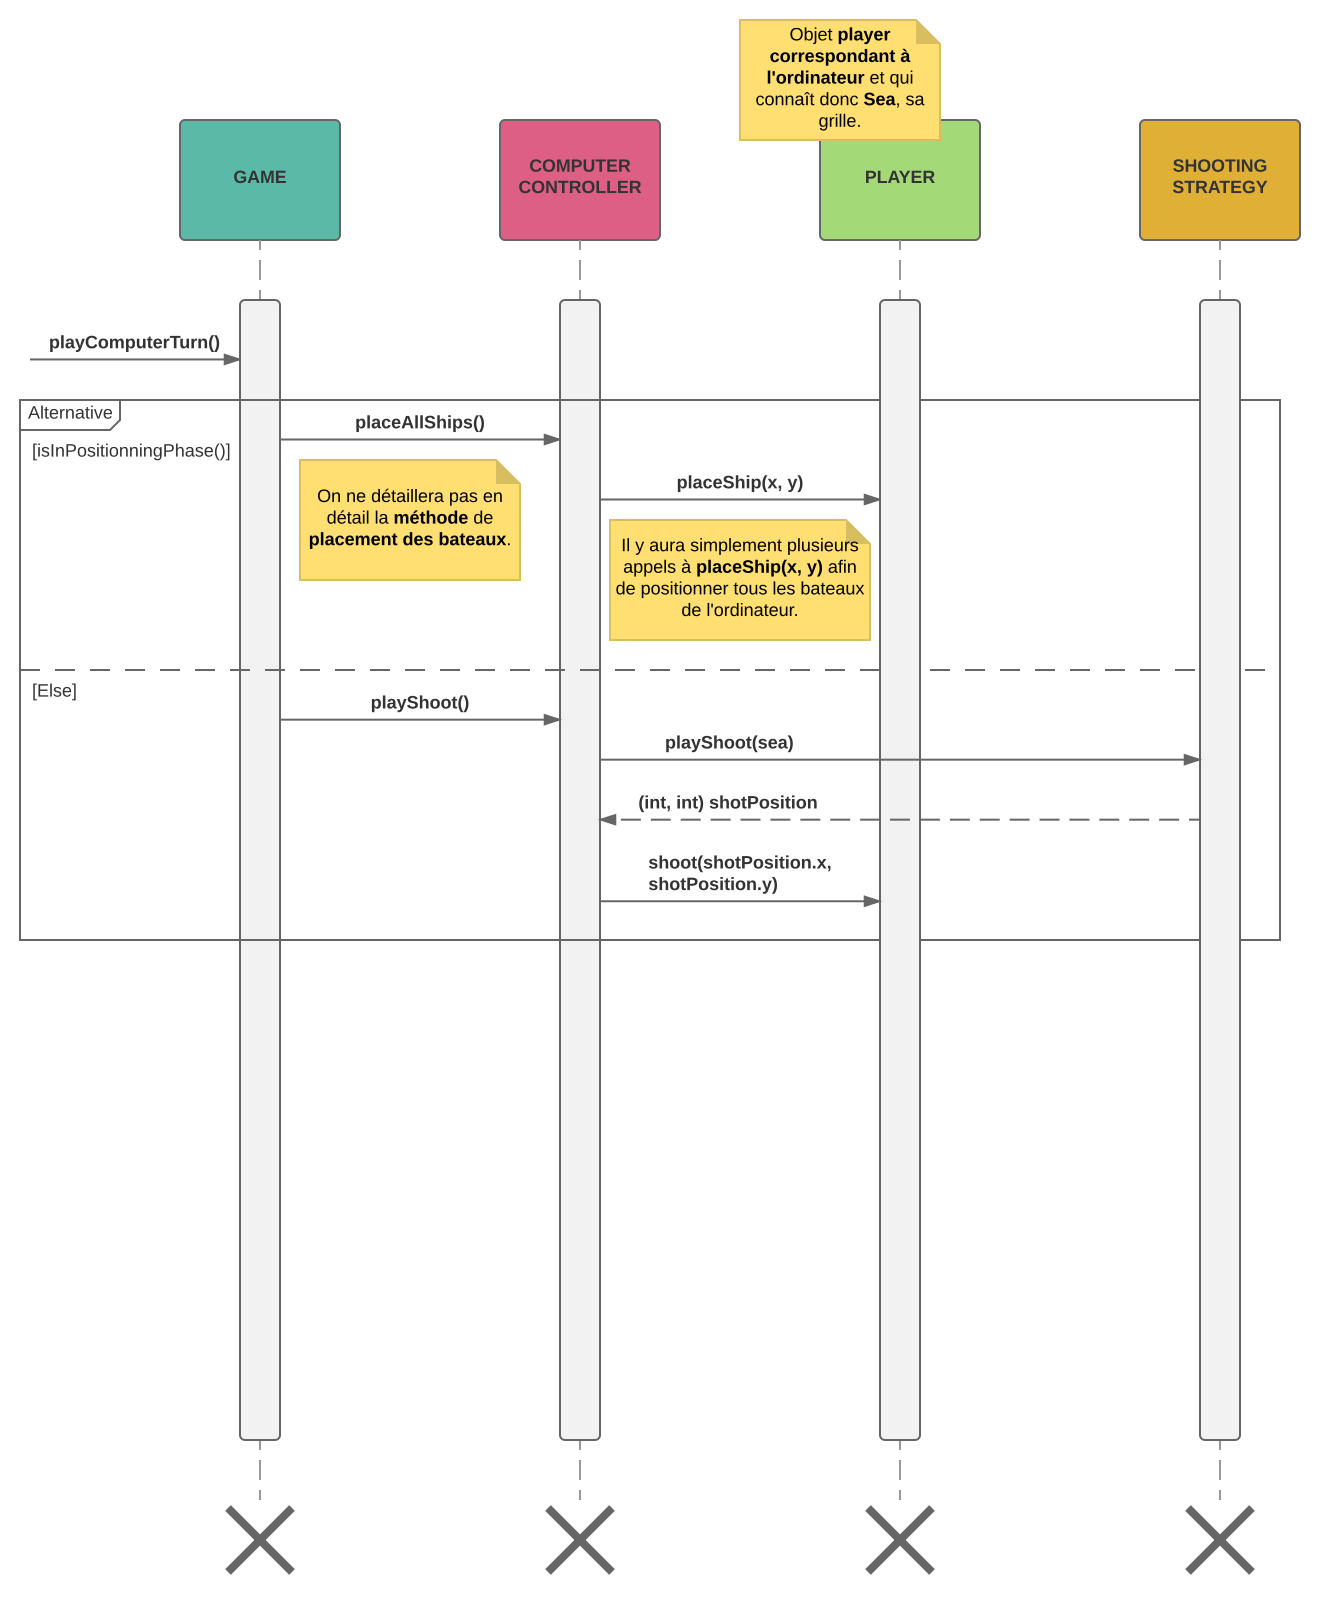
\includegraphics[width=\textwidth]{./src/img/sequence-game-playcomputerturn.pdf}
	\caption{Diagramme de séquence - game.playComputerTurn()}
\end{figure}

\begin{figure}[h!]
	\centering
	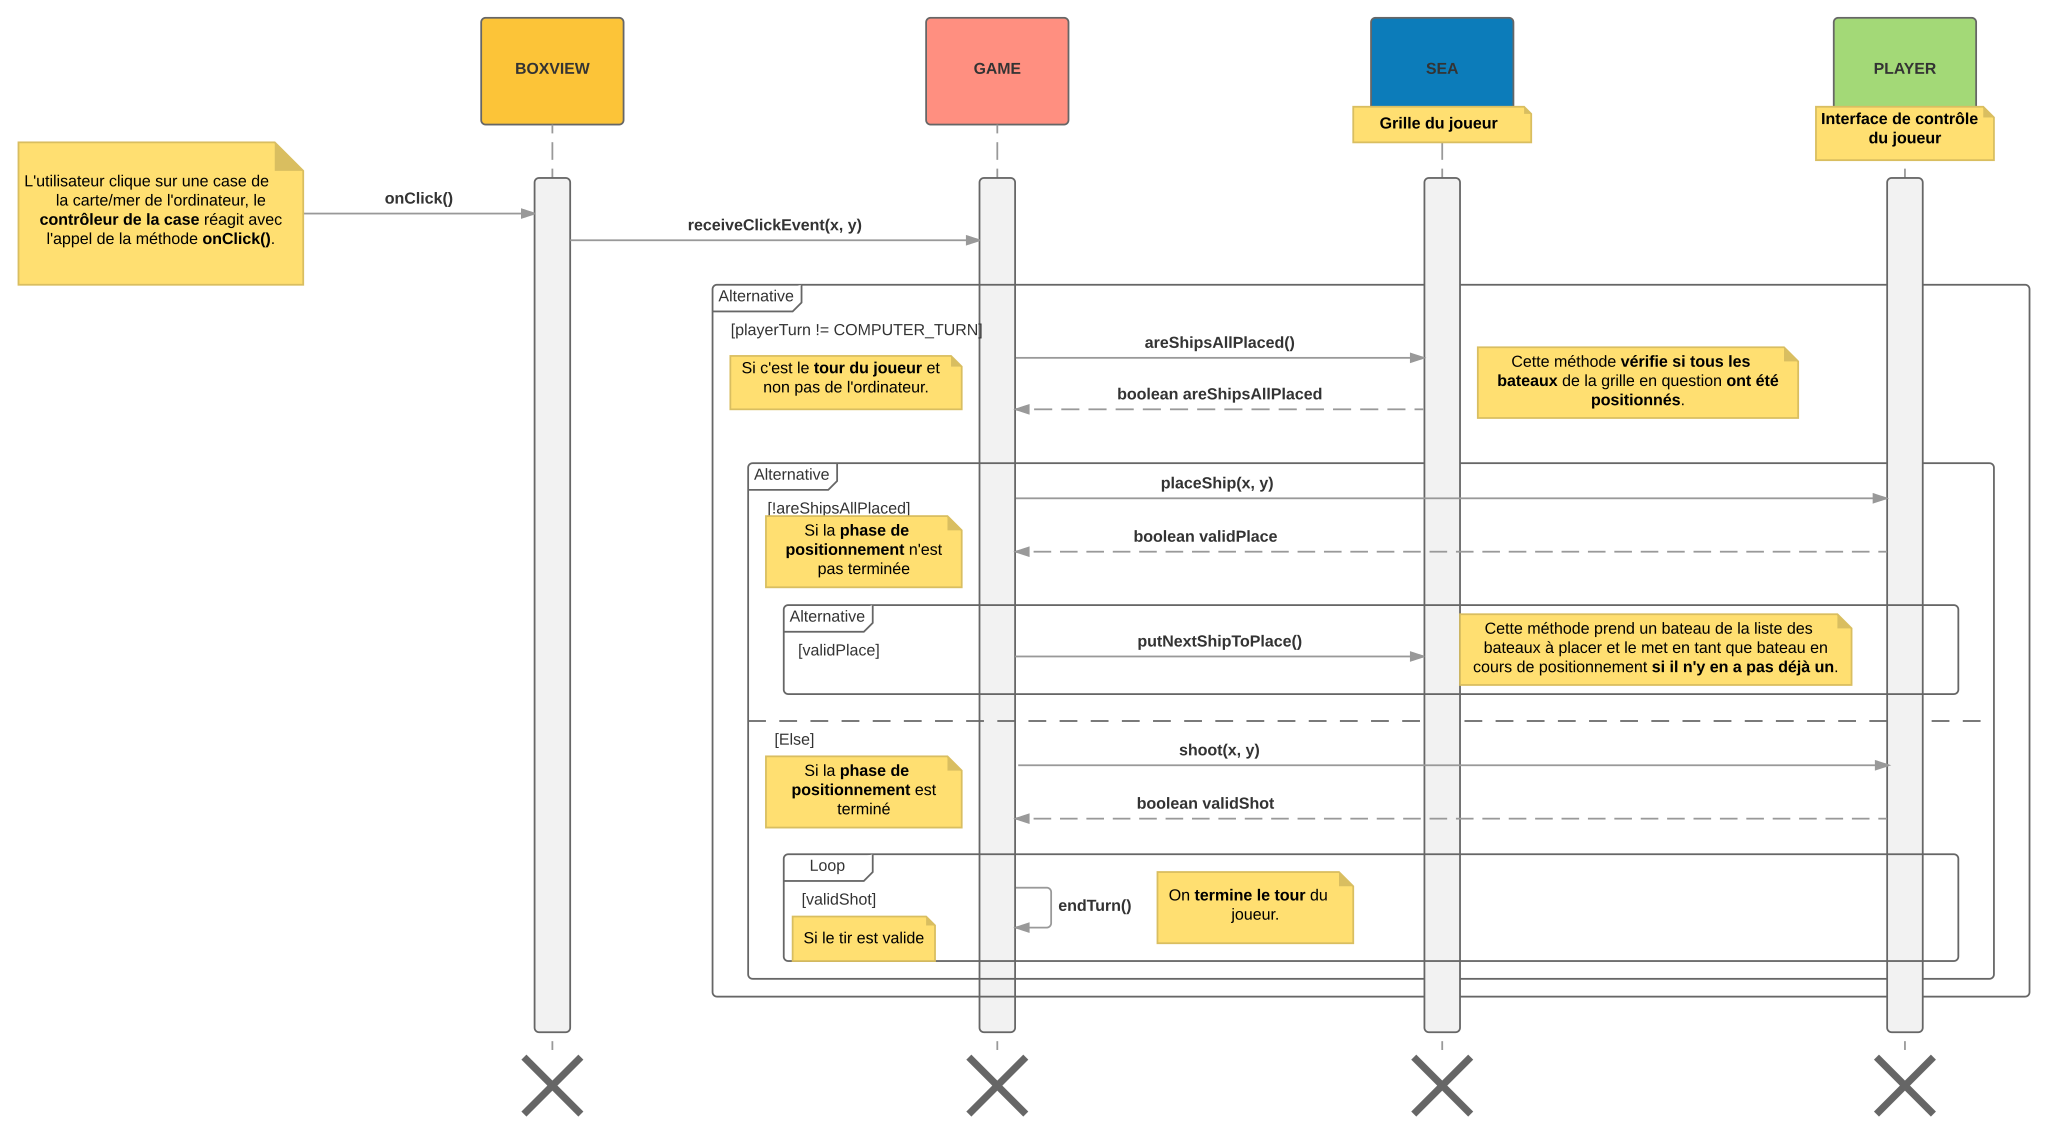
\includegraphics[angle=90, width=0.8\textwidth]{./src/img/sequence-game-receiveclickevent.pdf}
	\caption{Diagramme de séquence - game.receiveClickEvent()}
\end{figure}

\begin{figure}[h!]
	\centering
	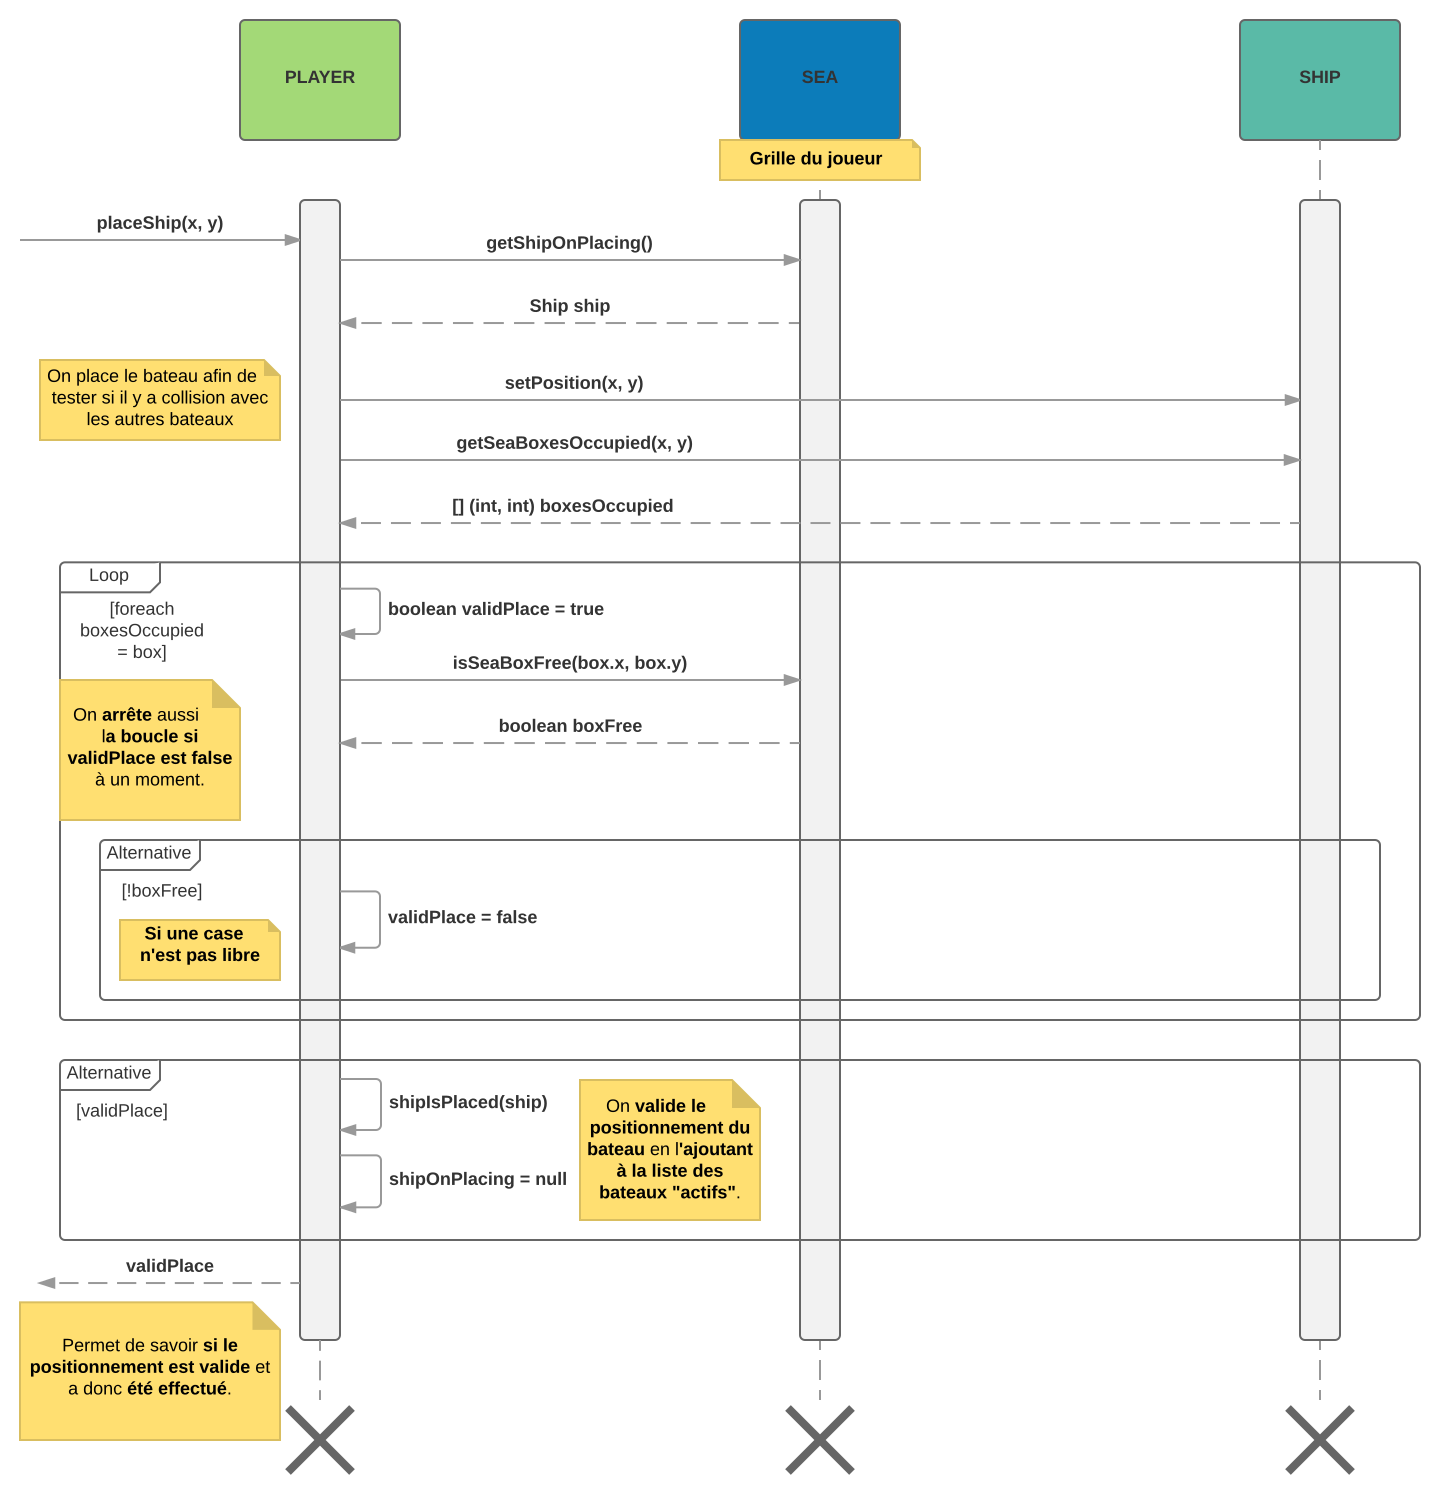
\includegraphics[width=\textwidth]{./src/img/sequence-player-placeship.pdf}
	\caption{Diagramme de séquence - player.placeShip()}
\end{figure}

\begin{figure}[h!]
	\centering
	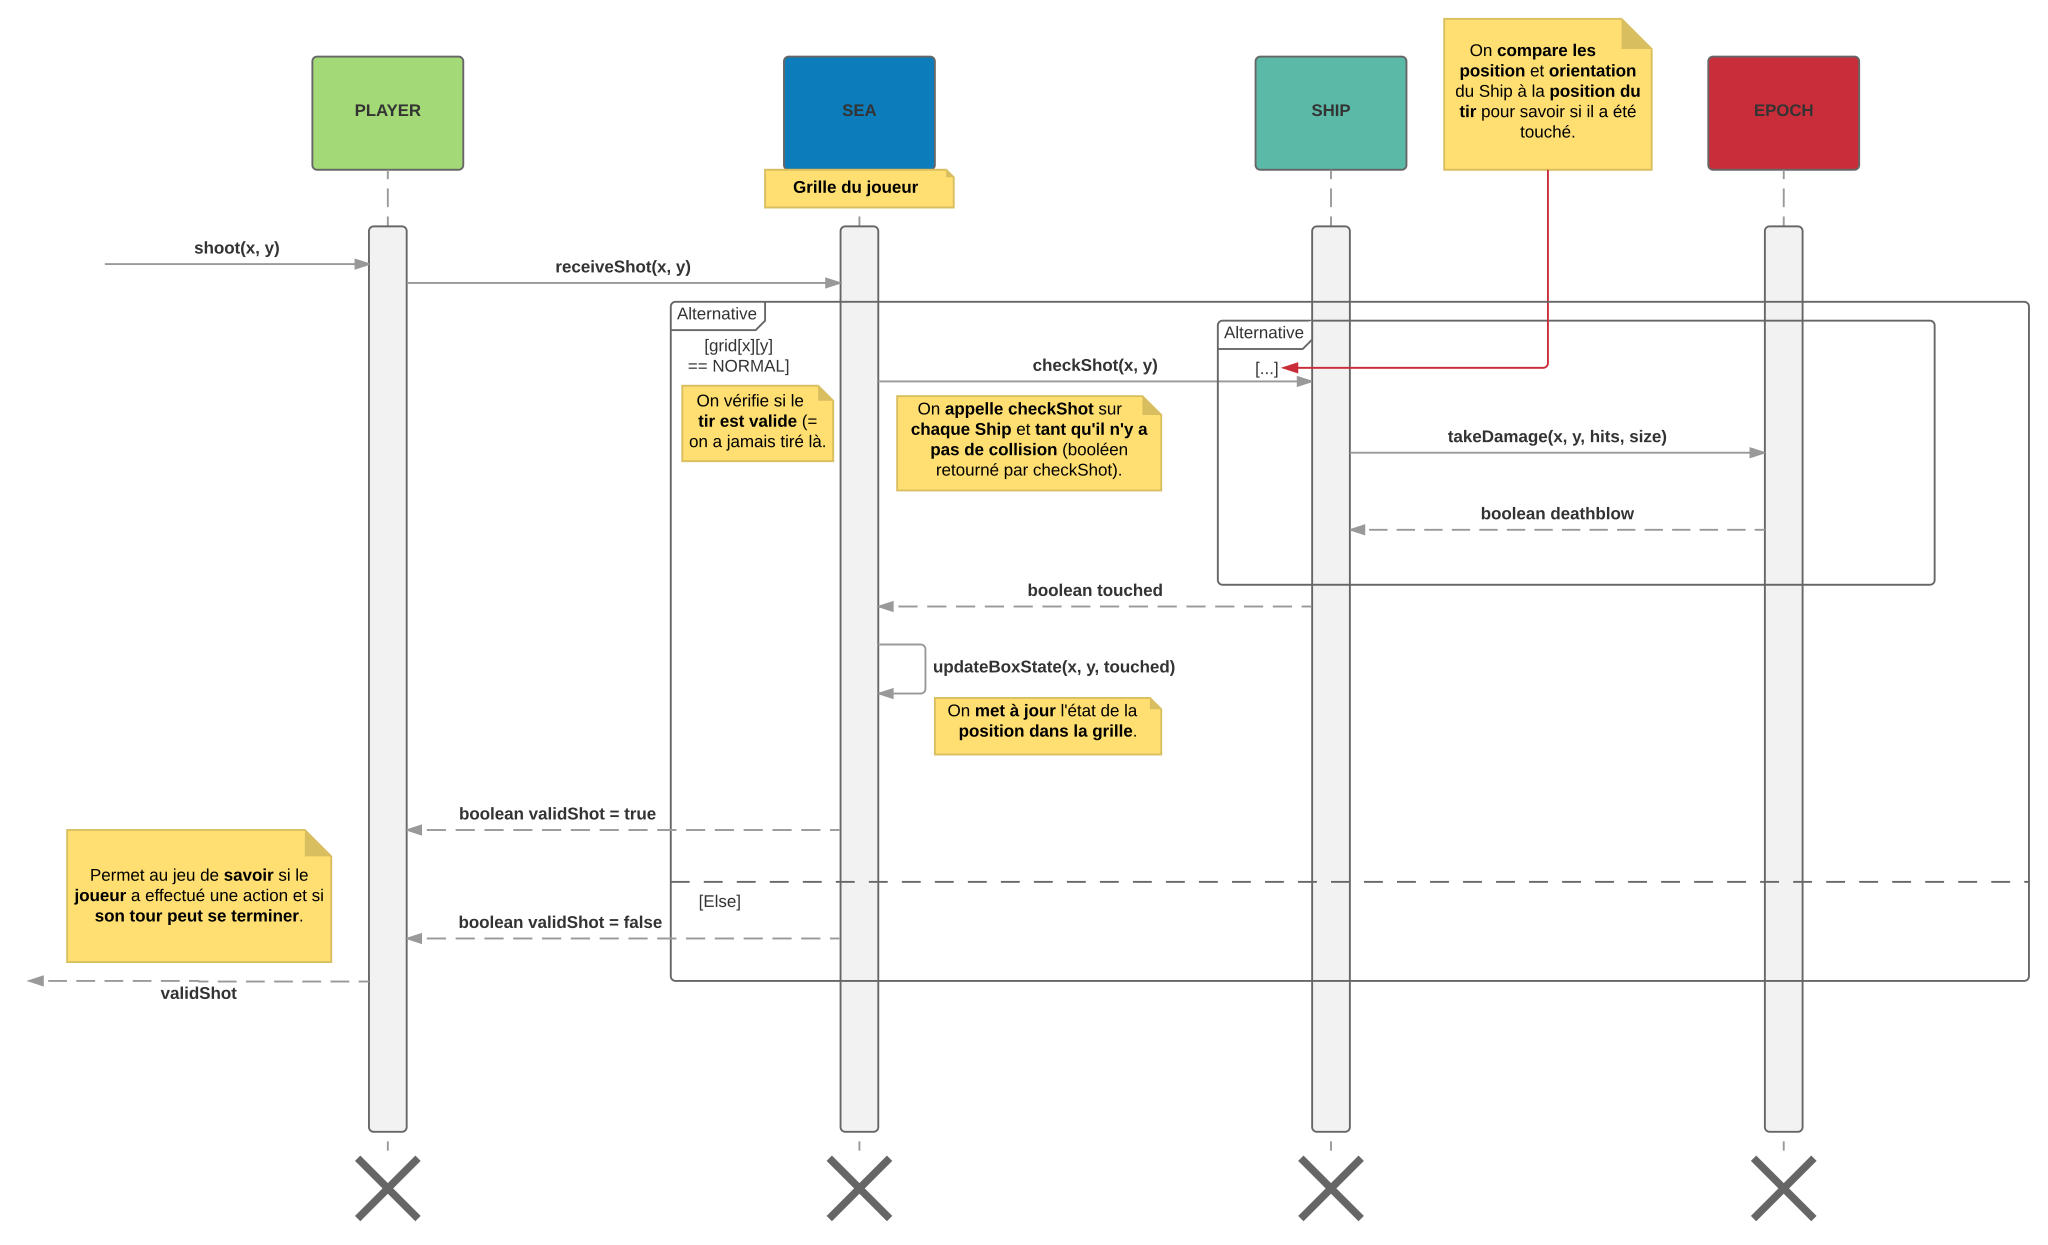
\includegraphics[angle=90, width=0.9\textwidth]{./src/img/sequence-player-shoot.pdf}
	\caption{Diagramme de séquence player.shoot()}
\end{figure}

\begin{figure}[h!]
	\centering
	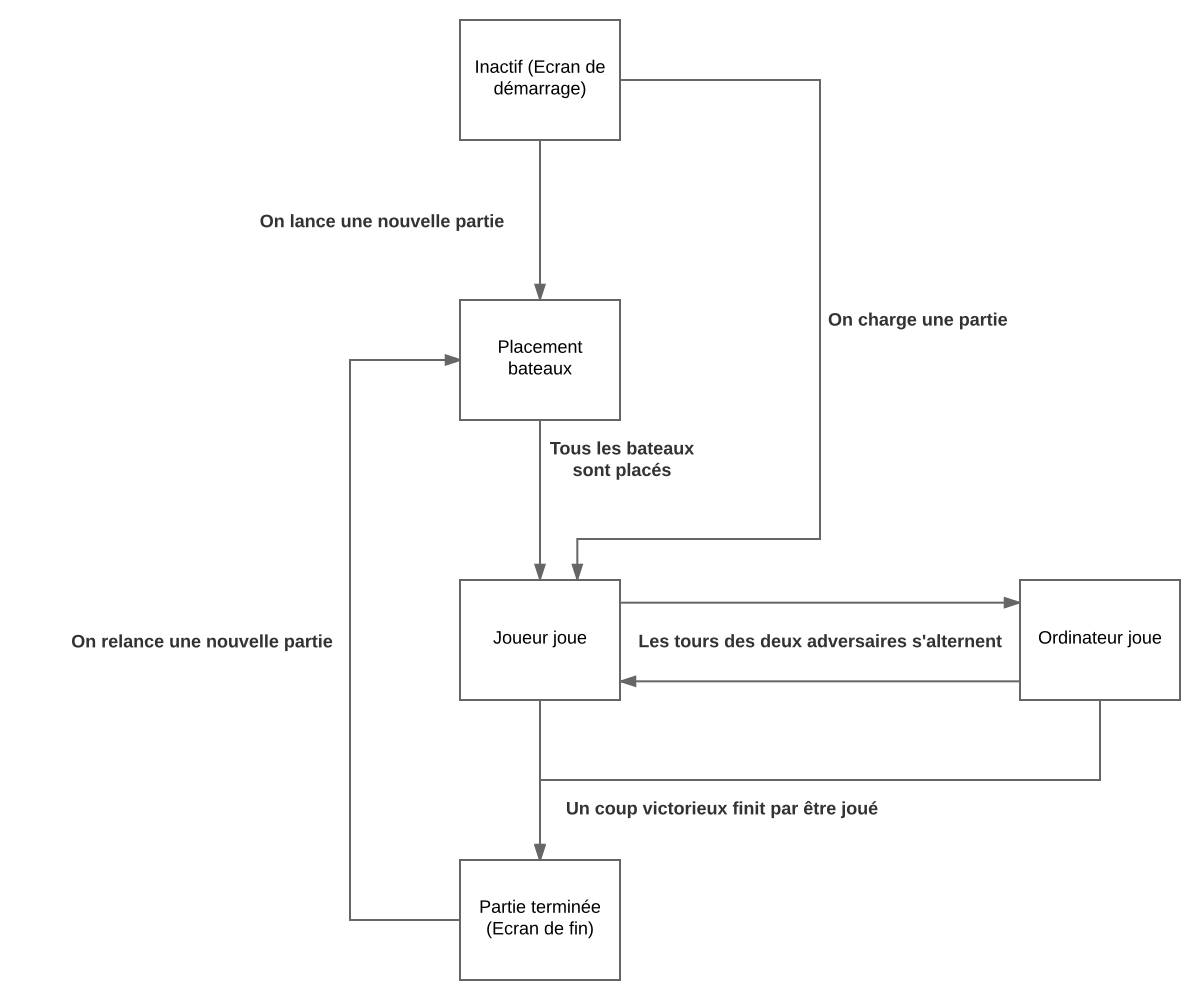
\includegraphics[width=\textwidth]{./src/img/etats.pdf}
	\caption{Diagramme d'états}
\end{figure}

\end{document}

% Mise en forme :

% \textbf{texte} -> gras
% \emph{text} -> italique
% \noindent -> supprimer l'indentation du prochain paragraphe
% \pagestyle{empty, plain, heading, myheadings} -> style de la page
% \thispagestyle{style} -> style de la présente page
% \renewcommand{\sectionmark}[1]{\markright{Partie \thepart, section \thesection : #1}{}} -> À utiliser dans le cas d'une style de page myheadings

% Autre :

% \addcontentsline{toc}{niveau}{nom} -> ajouter une ligne à la table des matières manuellement
% \setcounter{niveau}{numéro} -> changer la numérotation d'un niveau (ex: \setcounter{section}{0})
% \appendix -> passer aux annexes
% \href{url}{nom} -> lien hypertexte
% \phantom{} -> espace vide (pour ne pas fusionner "--" par exemple)
% \shorthandoff{caractère} -> supprimer l'espace avant/après un caractère

% Mesures :

% \textwidth -> largeur du texte
% \linewidth -> longueur de la ligne

% Astuces :

% Pour bien placer les figures (si besoin) : \begin{figure}{h!} et \clearpage après la figure
